\section{Experiments}

\subsection{Implementation Details}
\label{sec:impl-deta}

We implemented three variants of algorithm (\ref{alg:dcsc}) for the cases $\ell = 1,2,3$. For the single layer case we let $W^T_1$ be a 11x11 convolution with striding of 2 and 8 filters. For $\ell = 2$ we let $W^T_{1}$ be an 11x11 convolution with 8 filters and $W^T_{1}$ be a 7x7 convolution with 16 filters. Finally for the $\ell = 3$ case: $W^T_{1}$ is an 11x11 convolution with 8 filters, $W^T_{2}$ is a 5x5 convolution with 16 filters, and $W^T_{3}$ is a 3x3 convolution with 32 filters. For both $\ell = 2$ and $\ell = 3$, all convolutions have striding of 2. For the single layer case we learned the dictionaries with the number of iterations set to 5 and then at test time increased the number of iterations to 20. For the two and three layer cases the number of iterations was fixed at train and test time to 10 except in section \ref{sec:effect-iter-optim} where the number of test and training iterations is varied. All training was done with the ADAM optimizer with the default parameters.
\subsection{KITTI Depth Completion Benchmark}
\label{sec:kitti-depth-compl}
% \begin{figure}
\begin{table}
\centering
\begin{tabular}{r|cc}
  \label{table:kitti}
  & RMSE (m) & MAE (m)\\\hline
  Bilateral NN~\cite{} & 4.19 & 1.09\\
  SGDU~\cite{} & 2.5 & 0.72\\
  Fast Bilateral Solver~\cite{} & 1.98 & 0.65\\
  TGVL~\cite{} & 4.85 & 0.59\\\hline
  Closest Depth Pooling & 2.77 & 0.94\\
  Nadaraya Watson~\cite{} & 2.99 & 0.74\\
  ConvNet & 2.97 & 0.78\\
  ConvNet + mask & 2.24 & 0.79\\
  SparseConvNet~\cite{} & 1.82 & 0.58\\
  Ma \& Karaman & 1.68 & 0.70\\\hline
  Ours 1 Layer & 2.77 & 0.83\\
  Ours 2 Layers & 1.44 & 0.47\\
  Ours 3 Layers & \textbf{1.35} & \textbf{0.43}\\
  \hline
 \end{tabular}
 \caption{Validation error of various methods on the KITTI Depth Completion benchmark. All resulsts except for SparseConvNet and Ma's are taken as reported from ~\cite{}. Our method outperforms all previous state-of-the-art depth only completion methods (Middle) as well as those that use RGB images for guidance (Top).}
\label{fig:kitti}
\end{table}



% \end{figure}

The KITTI dataset provides raw LIDAR measurements in conjunction with high resolution RGB images from 22 video sequences of driving in both cities and highways. Combining all video sequences gives 93k frames with semi-dense ground truth depth. However, these measurements are corrupted by noise, motion of the vehicle during sampling, and image rectification artifacts. Additionally the raw LIDAR points are very sparse, accounting for only 4\% of the total number of pixels in the map. For these reasons the raw KITTI dataset is not ideal for evaluating depth completion systems.\\

The sparsity issue can be resolved by accumulating LIDAR measurements from nearby frames in the video sequences, and by using semi-global matching to reconstruct dense 3D points which can be projected using the given calibration files. Both these processes introduce more errors from occlusion and non-rigid movement across frames. Urhig \etal resolved these issues by automatically removing accumulated LIDAR points that deviate too far from the SGM points. The result is the KITTI depth completion benchmark, the first and only large scale dataset for depth completion training and evaluation. This benchmark is ideal since it has high quality ground truth and effectively simulates the main application of depth completion: recovering dense depth from a single LiDAR sweep.\\

Urhig \etal then evaluated their proposed Sparsity Invariant CNNs on this dataset as well as several other current methods for depth completion. Figure (\ref{fig:kitti}) shows the results they present along with our method and the results of the very deep Sparse-to-Dense network proposed by Ma \& Karaman. The Sparse-to-Dense network is fairly standard, using Resnet-18 as an encoder and up-projection blocks for a decoder. Similar architectures have been presented in other works for single shot depth prediction. While the deep Sparse-to-Dense network is able to achieve good RMSE, it fails to out perform the SparseConvNet on MAE. We believe that this is because the deeper network can better estimate the average depth of a region but is unable to predict fine detail, leading to a higher MAE. By comparison, our method is able to both estimate the correct average depth and reconstruct fine detail due to its ability to directly optimize the prediction with respect to the input. Most notably our method outperforms all of the existing methods by a wide margin, including those that use RGB images and those that use orders of magnitude more parameters than our method.
\subsection{Effect of Amount of Training Data}
\label{sec:effect-training-data}
\begin{figure}
\centering
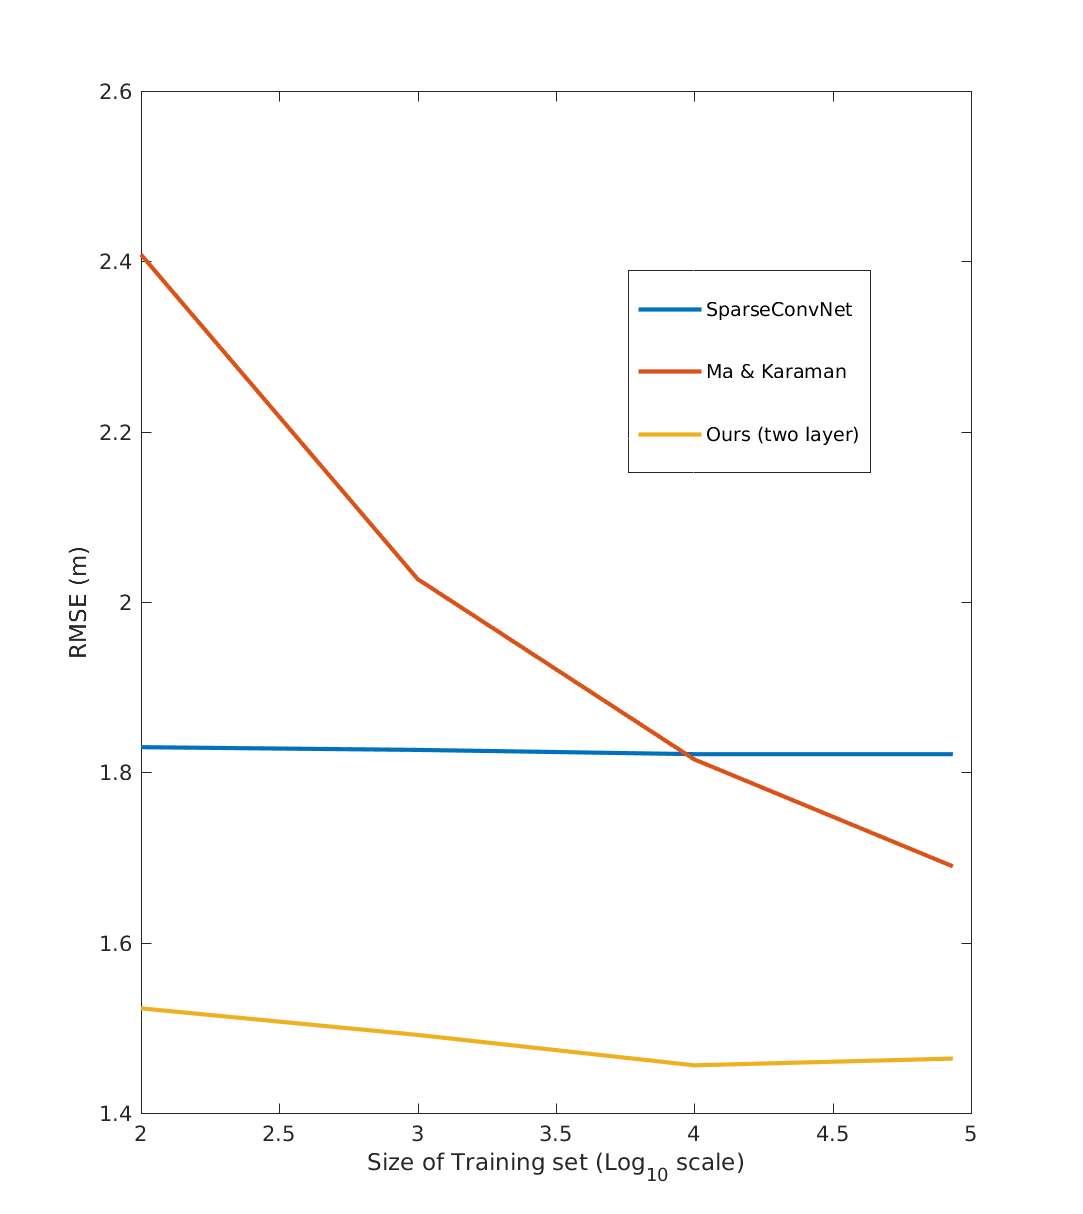
\includegraphics[width=0.45\textwidth]{trainsizeplot}
  \caption{Results of selected methods for varying training set sizes.}
  \label{fig:trainsize}
\end{figure}
Modern deep learning models typically have tens of thousands to millions of parameters and therefore require enormous training sets to achieve good performance. This is in fact the motivation for the KITTI depth completion dataset, since previous benchmarks did not have enough data to train deep networks. In this section we investigate the dependence on the amount of training data on the performance of our method in comparison with a standard deep network and the sparsity invariant variety.\\
Figure (\ref{fig:trainsize}) shows the results of evaluating these models on the 1k manually selected validation depth maps after training on varying subsets of the 86k training maps. Our method outperforms both baselines for all training sizes. As expected Ma \& Karaman's method fails to generalize well when trained on a small dataset since the model has ~3.4M parameters but performs well once trained on the full dataset. It is interesting to observe that the method of Urhig \etal does not gain any performance from training on more data. Our method is able to perform comparably to the sparsity invariant network with only 100 training examples but does increase in performance when given more data, validating the need for learning layered sparse coding dictionaries from large training sets. 
\subsection{Effect of Iterative Optimization}
\label{sec:effect-iter-optim}
\begin{figure}
  \centering
  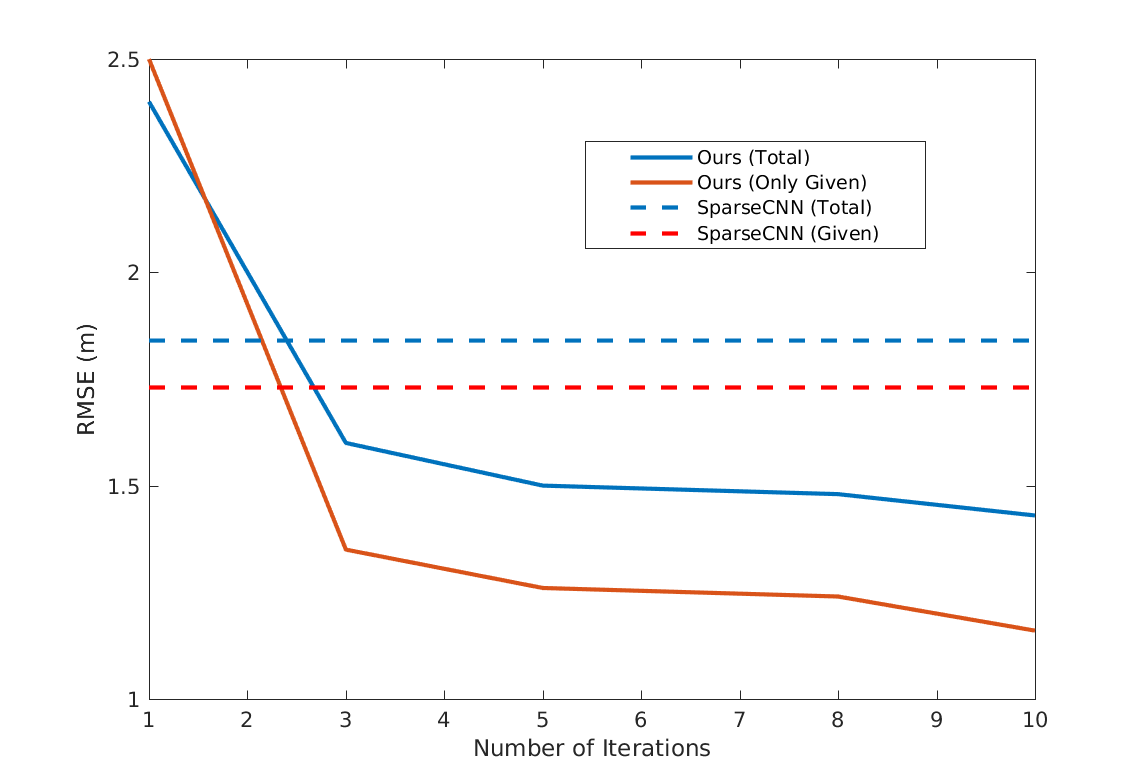
\includegraphics[width=0.45\textwidth]{iterplot}
  \caption{Results on the depth completion benchmark for different numbers of ADMM iterations. The total error is shown in blue while the red line shows the error on just those points given as input. The dotted lines show the same metrics but for the SparseConvNet of Urhig \etal}
  \label{fig:iterplot}
\end{figure}

In this section we demonstrate that the success of our approach comes from its ability to refine depth estimates over multiple iterations. Applying a feed forward neural network to this problem frames it as finding a mapping from sparse LiDAR points to true depth maps. This is a reasonable approach but it doesn't utilize all of the available information, specifically it doesn't encode the relationship that input samples are a subset of the output. In contrast, our approach of phrasing depth completion as a compressed sensing missing data problem directly expresses that relationship. By solving this problem in an iterative fashion our network that is able to find depth maps that are both consistent with the input constraints and have sparse representations.\\

The importance of iterative optimization is shown in Figure (\ref{fig:iterplot}) where we examine the performance of our method as a function of the number of ADMM iterations it uses. It is clear that with few iterations our network fails to enforce the constraints and performs comparably to the SparseConvNet. This is also consistent with Murdock \etal's observation that a feed forward network resembles a single iteration of an ADNN. As we increase the number of iterations our method is able to better optimize its prediction and gains a substantial performance boost.
% - Feed-forward is bad for this problem
% - Phrasing it as optimization is better, specifically sparse coding
% - All the best algorithms for CSC require multiple iterations to converge to a good solution
% - We have evidence for this, more iteration decreases both the total error and the error on the constraint points

% - instead of viewing problem as mapping from sparse input to dense depth we define it as an optimization problem over the given depth values and their sparse codes.
% - 


